\chapter{Problem Analysis}\label{ch:probdesc}



\section{Photovoltaic power}
While plants using fossil fuels or nuclear power are outputting high voltage AC directly into the grid, the renewable sources need to be boosted to high voltage, before they can feed their energy into the grid. 
Especially Solar panels produce very low power DC-voltage. \todo[color=c01]{ref}
% https://panasonic.net/ecosolutions/solar/product/product_detail/index.html

The setup to supply the energy to the grid can be seen in Figure \ref{fig:SolarConverters}.
There are three stages between converting solar to electric power and inputting that power into the grid. 
First, the low voltage DC coming in from the panel needs to be boosted, before an inverter makes it alternating. Finally  an AC-AC converter 

This three steps involve complicated circuitry, large costs and significant power losses. 
This remains one of the big reasons why solar power is not as cost efficient as other sources that do not require such conversion.

\begin{figure}[H]
   \centering
   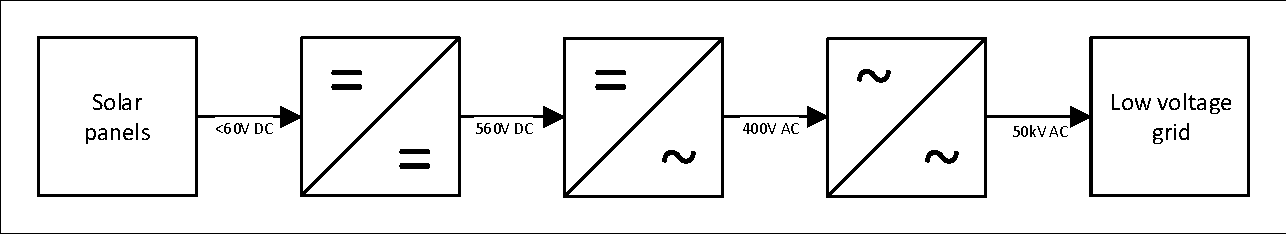
\includegraphics[width=\textwidth]{figures/Problem/SolarConverters.pdf}
    \caption{Connection of solar panels to the grid}
	\label{fig:SolarConverters}
\end{figure}

\section{Problem Description}
This project will focus on trying to improve the first stage or the DC-DC converter. 
The challenge for the boost converter is that the difference is very big.
A typical output of a solar panel is up to 60V DC while the low voltage grid is already 400V AC.
By connecting more panels in series a higher output voltage can be achieved but the power of individual panels can't be used as efficiently.
Using boost converters is the better solution but the standard boost converter topology is not suitable for this case. 
The maximum conversion ratio of the standard converter is limited to a ratio 7.7.
At least cascaded converters are needed to reach the higher internal voltage level.
But they still have to always run on high duty cycles to reach the demanded conversion ratios.
Advanced topologies have higher conversion ratios that may be useful for connecting solar panels.
In general new topologies for boost converters can have advantages over the conventional boost converters when it comes to compactness, efficiency and durability.

 
